Directional vector of a line1 having slope 2 is \myvec{1\\2}
    Hence normal vector of line$1$ is given as
\begin{align}
\vec{n_1} =\myvec{0 & -1\\1 & 0}\myvec{1\\2}\\=\myvec{-2\\1}
\end{align}
Similarly, normal vector for line 2 \\
\begin{align}
\vec{n_2} = \myvec{-m_2\\1}
\end{align}
Angle between two lines $\theta$ can be given by

\begin{align}
\cos \theta &= \frac{\vec{n_1}^T\vec{n_2}}{\norm{\vec{n_1}}\norm{\vec{n_2}}}\\
\implies \cos 60\degree &=\frac{1}{2}\\ 
=\frac{2m_2+1}{\sqrt5\times\sqrt{1+m_2}}
\end{align}
 \begin{align}
 \implies 11m_2^2+16m_2-1=0
 \end{align}
 Solving, m$_2$ yields values $\frac{-8+5\sqrt{3}}{11}$ and $\frac{-8-5\sqrt{3}}{11}$ \\
 Equation of line with normal vector $\vec{n}$ and passing through point A is given by
 \begin{align}
 \vec{n}^T(\vec{x}-A)=0
 \end{align}
  Hence,equation of line with slope $\frac{-8+5\sqrt{3}}{11}$ passing through \myvec{2\\3} is
  \begin{align}
  \myvec{\frac{8-5\sqrt{3}}{11}&1}\left(\vec{x}-\myvec{2\\3}\right)=0\\
  \implies \myvec{\frac{8-5\sqrt{3}}{11}&1}\vec{x}=\frac{49-10\sqrt{3}}{11}
  \end{align}
  Similarly,equation of line with slope $\frac{-8-5\sqrt{3}}{11}$ passing through \myvec{2\\3} is
  \begin{align}
  \myvec{\frac{8+5\sqrt{3}}{11}&1}\left(\vec{x}-\myvec{2\\3}\right)=0\\
  \implies \myvec{\frac{8+5\sqrt{3}}{11}&1}\vec{x}=\frac{49+10\sqrt{3}}{11}
  \end{align}
  Thus, the required line equations are
  \begin{align}
  \myvec{\frac{8-5\sqrt{3}}{11}&1}\vec{x}=\frac{49-10\sqrt{3}}{11}\\ 
%  \text{and}\hspace{10}
   \myvec{\frac{8+5\sqrt{3}}{11}&1}\vec{x}=\frac{49+10\sqrt{3}}{11}
  \end{align}
See Fig. \ref{Fig4:solutions/line_plane_40/}
\begin{figure}[!ht]
\centering
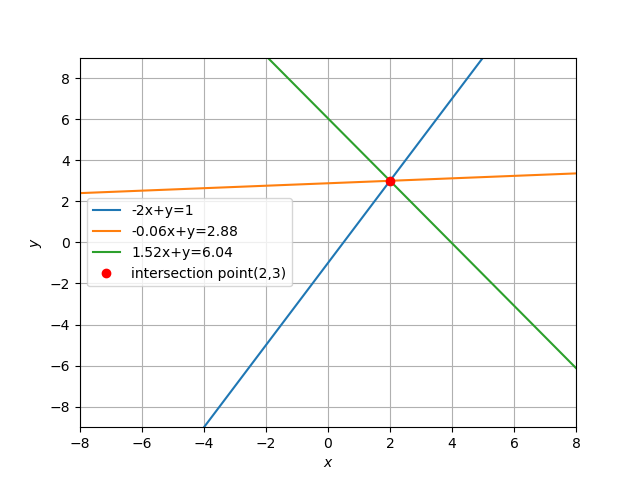
\includegraphics[width=\columnwidth]{./solutions/line_plane/40/plot.png}
\caption{plot showing intersection of lines}
\label{Fig4:solutions/line_plane_40/}
\end{figure}
